\chapter{Cambiamento di variabili negli integrali doppi (e multipli)}

\section{Concetto generale}
Dato il piano $xy$ e una certa figura $D$, immaginiamo di avere una funzione che mappa le coordinate:
\[
\begin{cases}
x = x(\xi, \eta) \\
y = y(\xi, \eta)
\end{cases}
\]
Questa applicazione mappa un dominio $\Omega \subset \mathbb{R}^2$ (nel piano $\xi\eta$) in un dominio $D \subset \mathbb{R}^2$ (nel piano $xy$).

Se abbiamo un'applicazione che soddisfa queste condizioni, quello che dobbiamo fare è indicare un punto in $(x, y)$ ed esprimerlo in coordinate $(\xi, \eta)$.

\subsection{Come traslano le coordinate?}
Se poniamo nel piano di partenza delle costanti:
\begin{itemize}
    \item $\eta = \text{costante} = \bar{\eta}$
    \item $\xi = \text{costante} = \bar{\xi}$
\end{itemize}
e prendiamo l'immagine di queste rette rispetto all'applicazione, otteniamo delle curve nel piano $xy$:
\begin{itemize}
    \item $\vec{r}(\xi, \bar{\eta}) \implies$ fisso $\bar{\eta}$ e faccio variare $\xi$.
    \item $\vec{r}(\bar{\xi}, \eta) \implies$ fisso $\bar{\xi}$ e faccio variare $\eta$.
\end{itemize}

\vspace{0.5cm}
\begin{center}
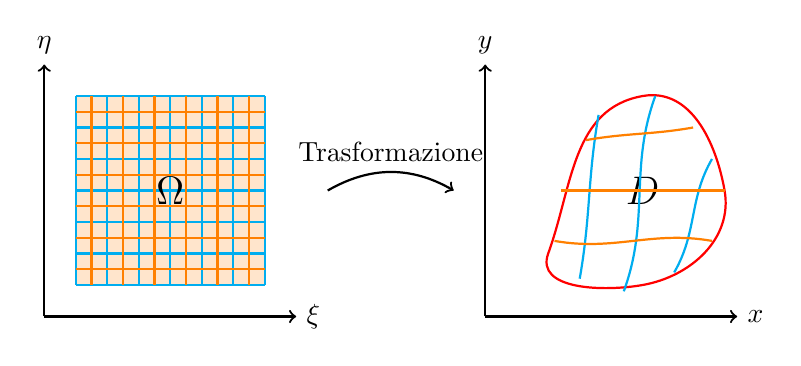
\begin{tikzpicture}[scale=0.8]
    % Piano \xi, \eta
    \begin{scope}[shift={(0,0)}]
        \draw[->, thick] (0,0) -- (4,0) node[right] {$\xi$};
        \draw[->, thick] (0,0) -- (0,4) node[above] {$\eta$};
        
        \fill[orange!20] (0.5,0.5) rectangle (3.5,3.5);
        \draw[step=0.5, cyan, thick] (0.5,0.5) grid (3.5,3.5);
        \draw[step=0.5, orange, thick, yshift=0.25cm, xshift=0.25cm] (0.25,0.25) grid (3.25,3.25);
    \end{scope}
    \node at (2, 2) {\Large $\Omega$};

    % Freccia trasformazione
    \draw[->, thick, bend left] (4.5, 2) to node[midway, above] {Trasformazione} (6.5, 2);

    % Piano x, y
    \begin{scope}[shift={(7,0)}]
        \draw[->, thick] (0,0) -- (4,0) node[right] {$x$};
        \draw[->, thick] (0,0) -- (0,4) node[above] {$y$};
        
        % Dominio D distorto
        \draw[thick, red] (1,1) to[out=70,in=190] (2.5,3.5) to[out=10,in=100] (3.8,2) to[out=-80,in=10] (2.5,0.5) to[out=-170,in=-110] (1,1);
        \node at (2.5, 2) {\Large $D$};
        
        % Curve trasformate
        \draw[cyan, thick] (1.5, 0.6) to[out=80,in=-100] (1.8, 3.2);
        \draw[cyan, thick] (2.2, 0.4) to[out=70,in=-110] (2.7, 3.5);
        \draw[cyan, thick] (3.0, 0.7) to[out=60,in=-120] (3.6, 2.5);
        
        \draw[orange, thick] (1.1, 1.2) to[out=-10,in=170] (3.6, 1.2);
        \draw[orange, thick] (1.2, 2.0) to[out=0,in=180] (3.8, 2.0);
        \draw[orange, thick] (1.6, 2.8) to[out=10,in=190] (3.3, 3.0);
    \end{scope}
\end{tikzpicture}
\end{center}

\section{Coordinate polari}
Le equazioni di trasformazione per le coordinate polari sono:
\[
\vec{r}(\rho, \theta) \implies 
\begin{cases}
x(\rho, \theta) = \rho \cos\theta \\
y(\rho, \theta) = \rho \sin\theta
\end{cases}
\qquad 
\left| \frac{D(x,y)}{D(\rho,\theta)} \right| = \rho
\]
Se da coordinate cartesiane voglio passare a polari, utilizzo:
\[
\rho = \sqrt{x^2 + y^2}, \qquad \theta = \arctan\left(\frac{y}{x}\right)
\]

\section{Applicazione del cambiamento di variabili}
Applicando la logica delle coordinate polari, la definizione dell'integrale doppio diventa:
\[
\lim_{\text{diam} \to 0} \sum_{i=1}^{N} f(P_i) \cdot \text{Area}(D_i)
\]
Questo ci porta a dire che l'area infinitesima della regione curvilinea $D_i$ nel piano $xy$ si può approssimare come:
\[
\text{Area}(D_i) \approx \text{Area del parallelogramma}
\]
L'area del parallelogramma formata dai vettori $\vec{r}_\xi \Delta\xi$ e $\vec{r}_\eta \Delta\eta$ è pari al modulo del loro prodotto vettoriale:
\[
\text{Area} = \|\vec{r}_\xi \Delta\xi \times \vec{r}_\eta \Delta\eta\|
\]

La matrice Jacobiana della trasformazione $(\xi, \eta) \to (x, y)$ è:
\[
J(x,y) = 
\begin{bmatrix}
\frac{\partial x}{\partial \xi} & \frac{\partial x}{\partial \eta} \\
\frac{\partial y}{\partial \xi} & \frac{\partial y}{\partial \eta}
\end{bmatrix}
\]
Il cui determinante (o Jacobiano) si indica convenzionalmente con la notazione: $\frac{D(x,y)}{D(\xi,\eta)}$.

Tutto questo ci porta a riscrivere l'integrale doppio in coordinate trasformate nella forma:
\[
\iint_D f(x,y) \, dx dy = \iint_\Omega f(x(\xi,\eta), y(\xi,\eta)) \left| \frac{D(x,y)}{D(\xi,\eta)} \right| d\xi \, d\eta
\]

\section{Coordinate nello spazio}

\subsection{Coordinate cilindriche}
L'estensione in tre dimensioni tramite le coordinate cilindriche è:
\[
\begin{cases}
x = \rho \cos\theta \\
y = \rho \sin\theta \\
z = z
\end{cases}
\implies \left| \frac{D(x,y,z)}{D(\rho,\theta,z)} \right| = \rho
\]

\subsection{Coordinate sferiche}
Utilizzando il raggio $R$, l'angolo di elevazione $\theta$ e l'azimut $\varphi$, si ottiene:
\[
\begin{cases}
x = R \cos\theta \cos\varphi \\
y = R \cos\theta \sin\varphi \\
z = R \sin\theta
\end{cases}
\implies \left| \frac{D(x,y,z)}{D(R,\theta,\varphi)} \right| = R^2 \cos\theta
\]
Con i limiti di integrazione standard per questa specifica notazione:
\[
\theta \in \left[-\frac{\pi}{2}, \frac{\pi}{2}\right], \qquad \varphi \in [0, 2\pi]
\]

\vspace{0.5cm}
\begin{center}
\begin{tikzpicture}[scale=1.5]
    % Assi 3D
    \draw[->, thick] (0,0,0) -- (3,0,0) node[right]{$y$};
    \draw[->, thick] (0,0,0) -- (0,3,0) node[above]{$z$};
    \draw[->, thick] (0,0,0) -- (0,0,4) node[below left]{$x$};

    % Coordinate del punto
    \coordinate (O) at (0,0,0);
    \coordinate (P) at (2, 2.5, 2);
    \coordinate (Pproj) at (2, 0, 2);

    % Vettori
    \draw[->, red, thick] (O) -- (P) node[right, black]{$R$};
    \draw[->, green!60!black, thick] (O) -- (Pproj) node[below right, black]{$R' = \text{proiezione}$};
    \draw[dashed] (P) -- (Pproj);
    \draw[dashed] (P) -- (0, 2.5, 0);

    % Angolo phi (azimut sul piano xy)
    \draw[cyan, thick] (0,0,1.5) arc [start angle=250, end angle=325, radius=1.5cm];
    \node[cyan] at (1, 0, 1.8) {$\varphi$};
    
    % Angolo theta (elevazione)
    \draw[orange, thick] (1.3, 0, 1.3) arc [start angle=-10, end angle=55, radius=1.5cm];
    \node[orange] at (1.5, 0.8, 1.3) {$\theta$};
    
\end{tikzpicture}
\end{center}